In this chapter, we present the vision that we defend in this document.
We first summarise the challenges addressed and our review of the state-of-the-art.
Then, we describe our vision.

\section{Summary of previous chapter}
\Glspl{adptSyst} engineer can use the \gls{mde} methodology to design the adaptation process \cf \Cref{chapt:intro}).
Among the open challenges we identified for this method, this thesis tackles the followings:
\begin{itemize}
	\item How to ease the manipulation of data uncertainty for software engineers?
	\item How to enable reasoning over unfinished actions and their expected effects? (\glspl{longTermAct})
	\item How to model the decisions of an adaptation process to diagnose it?
\end{itemize}

We show in~\Cref{chapt:sota} that it exists no solution to model \gls{longTermAct} or to reason over them.
Besides, we establish that research efforts are still required to handle \gls{duc} at the language level.
To come to this conclusion, we perform a review driven by two research questions (\cf \Cref{sec:sota:methodo}):
\begin{itemize}
	\item \textit{[RQ1]} Do state-of-the-art solutions that model \glspl{adptSyst} allow representing and reasoning over long-term actions?
	\item \textit{[RQ2]} Do state-of-the-art solutions allow modelling uncertainty of data and its manipulation (propagation, reasoning over)?
\end{itemize}

\section{Vision}
\begin{figure}
	\centering
	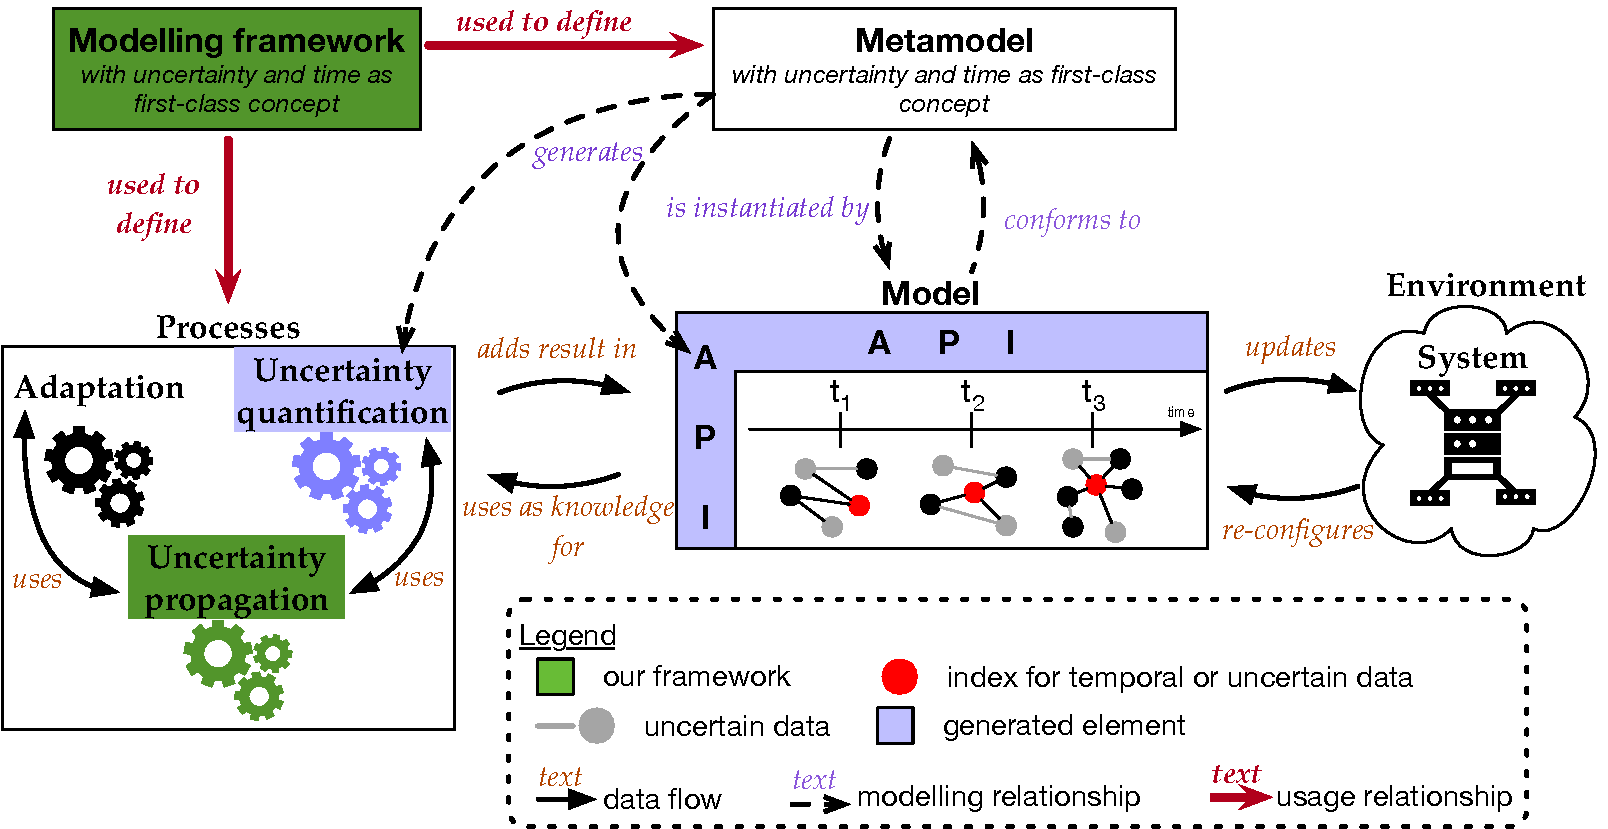
\includegraphics[width=\linewidth]{img/chapt-vision/vision}
	\caption{Overview of our vision}
	\label{fig:vision:vision}
\end{figure}

We think that both challenges can be addressed by the definition of a modelling framework that includes, besides all traditional elements, temporal and uncertainty as first-class concepts.
We depict this vision in~\Cref{fig:vision:vision}.
Using this framework, designers can define the structure of the data model, in the figure shown as the \gls{metamodel}, and the adaptation process.
The \gls{metamodel} contains high-level information about the time and uncertainty.
Based on this information, the uncertainty quantification process and a high-level API will be generated, both depicted in blue in the figure.
The process will read data of the model and add uncertainty information.
If we take a \gls{sg} example, when the system receives a consumption value, the process adds a probability distribution that represents the uncertainty of the value.
The uncertainty quantification process, as the adaptation process, uses a language with uncertainty and time as first-class citizens.
Therefore, they both use a process that automatically propagates uncertainty, which is part of our modelling framework.
The API generated from the \gls{metamodel} will help stakeholders to manipulate the model, conforms to the \gls{metamodel}.
This API will use specific indexes for temporal and uncertain data.
These indexes will help the manipulation of large models.
In the figure, we don't depict the storage mechanism nor the mechanism that load data.

Hartmann~\etal partially implemented this vision~\cite{DBLP:journals/is/HartmannFMRT19}, which led to the \gls{gcm}. 
Using this framework, a modeller will not specify any time-related information in the models.
They will be automatically generated by the framework, with dedicated data structures for temporal data to enable efficient storage and query.

We present, in this thesis, two contributions towards this vision.
First, we detail our language named \langName{}, which permits designers managing uncertainty at the language level, in~\Cref{chapt:aintea}.
We can assume that the language is part of the modelling framework, used to define reasoning processes such as the adaptation process.
This solution addressed the challenge of the manipulation of uncertain data (cf. Sub-Challenge \#1). 
Second, we describe a temporal knowledge model in~\Cref{chapt:tkm} to structure and store the state and behaviour of a running \gls{adptSyst}, with running \glspl{longTermAct}.
This model addresses the challenge of reasoning over unfinished actions, and understanding of \gls{adptSyst} \gls{behaviour} (cf. Sub-Challenge \#2 and \#3).
This \gls{metamodel} can be understood as an example of a result of our modelling framework.
\looseness-1


